\section[Script to Agent]{Script to Agent: From code to deployment}

This section describes the process of deploying a DSL script, from to code, to a functioning agent enforcing rules and generating reports.

\subsection{Compilation}

Deploying a script requires two outside interactions. The first is when the script is uploaded. The \ref{fig:seq0} figure shows how it is done.

\begin{figure}[h]
    \centering
    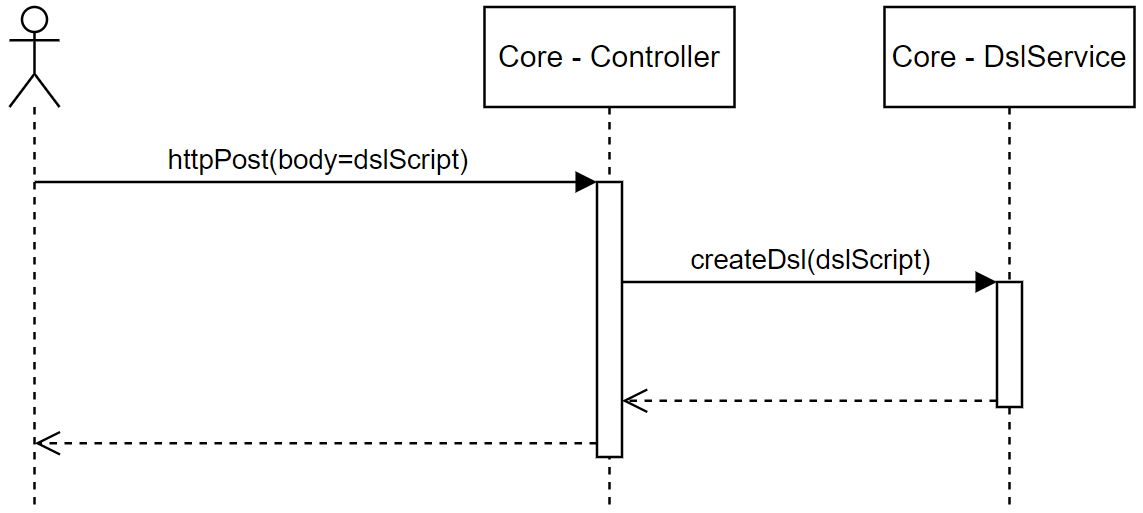
\includegraphics[width=130mm, keepaspectratio]{seq0.png}
    \caption{Upload script}
    \label{fig:seq0}
\end{figure}

During upload, the script file is embedded in the body of an HTTP Post request. Konstrainer-Core is a multilayer application. The controller layer receives the Post request, extracts the file name as a String, and the file content as a ByteArray. After that, the `createDsl' function of the service layer is called, which persists the script and starts the compilation process. The \ref{fig:seq1} diagram explains what the `createDsl' function does.

\begin{figure}[h]
    \centering
    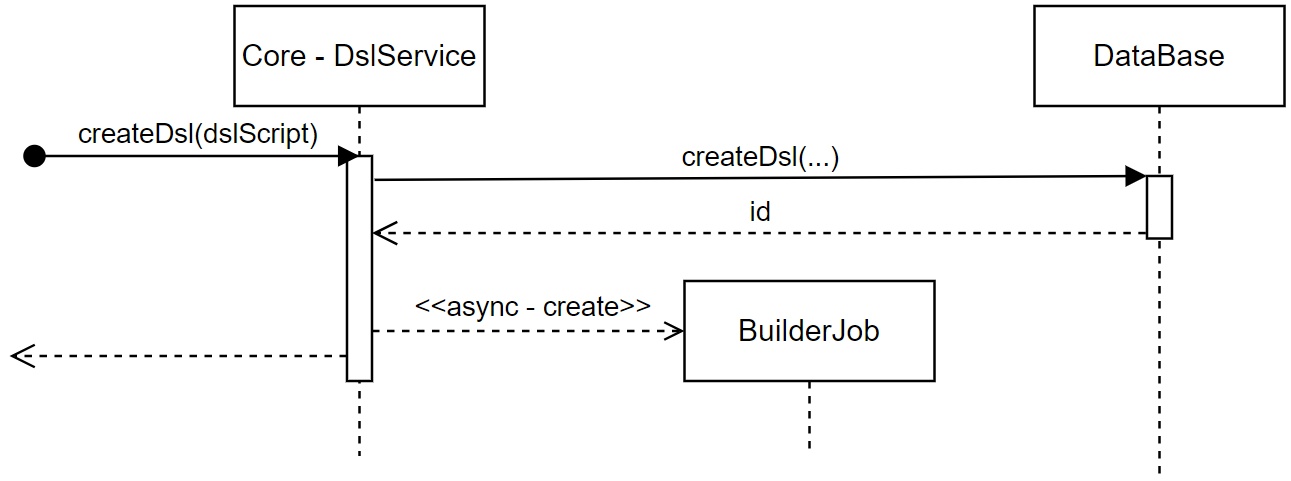
\includegraphics[width=130mm, keepaspectratio]{seq1.png}
    \caption{`createDsl' function}
    \label{fig:seq1}
\end{figure}

First, the `createDsl' function creates a new DSL record in the database. The filename, file content, and a timestamp is included in this record. A flag is also set that indicates the build status. At this point this flag is set to "Building", indicating that the compilation is in progress. The function that creates the database record returns the created object. The ID of this object is then extracted because the builder job uses it to reference the DSL script it needs to compile.

The compilation is run as a Kubernetes Job. The ID of the DSL script and the host address of the Core application are set as environment variables. The Builder and the Core communicate using HTTPS. The root CA of the Core app's certificate is mounted to the job on a volume, so it can be added to the trusted certificate authorities in that container. 

After the builder job is created in Kubernetes, the `createDsl' function returns, and the rest of the compilation is done asynchronously. The \ref{fig:seq2} figure explains process of compilation.

\begin{figure}[h]
    \centering
    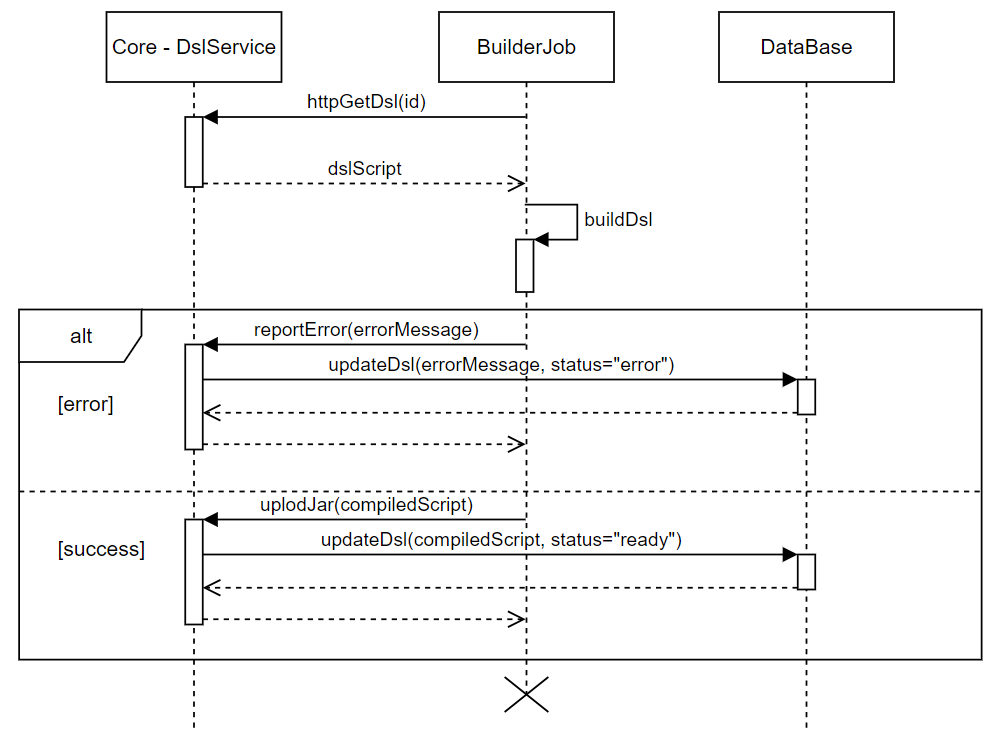
\includegraphics[width=130mm, keepaspectratio]{seq2.png}
    \caption{Script compilation}
    \label{fig:seq2}
\end{figure}

This detail is not marked on the diagram, but the Builder starts with adding the root CA of the Core app to its trusted certificate authorities. After this, it downloads the script as a text file. The Core app's API has an HTTP Get endpoint which enables the download of any script file by ID. After the file was successfully downloaded, the builder does some preprocessing on the file, and starts the Gradle build. 

If the build succeeds, the compiled jar is uploaded to the Core server, which will first load it, to extract some metadata, than save it to the database. In this case the following updates will occur on the database record:

\begin{minipage}{\linewidth}
\begin{itemize}
    \item The name of the script will be updated from the filename, to the server name defined in the script.
    \item The compiled jar will be added to the record.
    \item The build status flag will be set to "Ready".
    \item A boolean flag is set whether the script has a report block.
    \item A boolean flag is set whether the script has webhooks.
\end{itemize}
\end{minipage}

In case of an error, an error message is sent, and the following changes will take place on the record in the database:

\begin{minipage}{\linewidth}
\begin{itemize}
    \item The build status flag will be set to "Failed".
    \item The error message will be saved.
\end{itemize}
\end{minipage}

\subsubsection{Builder job detailed implementation}

The builder job is implemented as a well-written Bash script. How I managed to implement error handling in Bash is quite interesting, so in this subsection, I will delve into the details of the builder script.

The builder image is built on top of the agent image, so it has exactly the same packages installed. Therefore, it is almost certain that if the builder can compile a script, the agent can run it too.

The builder image also includes a prepared Gradle project with an empty script in it. During the build of the Docker image, this empty script is compiled using Gradle, so everything that can be cached, is cached, drastically decreasing the compilation time. Before this optimization, the compilation took about 3 minutes, now it takes only 40 seconds.

The \ref{code:builder0} code snippet show the important parts of the builder script, however the entire script can be found in the appendix, referenced by: \ref{appendix:builder} \nameref{appendix:builder}. Some lesser important details are replaced by dots: `\dots'

\begin{minipage}{\linewidth}
\begin{lstlisting}[caption={Builder script},language=bash,label=code:builder0]
cp "/app/tls-cert/rootCa.pem" /usr/local/share/ca-certificates/rootCa.crt
update-ca-certificates

echo "=== BEGIN ERROR REPORT ===" > $logsfile
function log() {
    echo "$1" >> $logsfile
}
    
function try_compile() {
    # Download script file
    wget ... && log "Download done" || \
        { log "Download failed" && error_report; }
    # Compile script
    ./gradlew jar >> $logsfile 2>&1 && log "Build done" || \
        { log "Build failed" && error_report; }
    log "Compilation done"
    # Upload compiled jar
    curl ... || { log "Upload failed" && error_report; }
}

function error_report() {
    log "=== END ERROR REPORT ==="
    # Send error report
    curl ...
    exit 1
}

try_compile || error_report
\end{lstlisting}
\end{minipage}

First, the trusted certificates are updated using the `update-ca-certificates' command from the `ca-certificates' Ubuntu package. The renaming of the certificate file is crucial because the `update-ca-certificates' command only adds certificates whose file extensions are `.crt'. Files with the `.pem' extension are ignored, a lesson I've learned the hard way.

The script is logging to a file, called `logsfile'. There are two main functions: `try\_compile' and `error\_report'. The last line of the script will execute the `try\_compile' function. If the function returns a non-zero status code, the `||' operator ensures, that the `error\_report' function is executed, which will finish the error report, and send it to the Core server. After sending the report, the job will exit with status code 1. This will also set the status of the Kubernetes job to failed.

Inside the `try\_compile' function, most commands are executed following the same pattern: \lstinline*command && log_success || { log_error && error_report; }* 

This pattern ensures that if the command succeeds, the fact of the success is logged. If the command returns a non-zero status code, it logs the failure, and invokes the `error\_report' function. The curly brackets are crucial because they do not create a new subshell. This means that the `exit 1' inside the `error\_report' will exit the entire scrip, instead of just exiting a subshell.

The call of the Gradle build on line 14 is unique. The \lstinline*./gradlew jar >> $logsfile 2>&1* bash magic appends the standard output (stdout) and the standard error (stderr) to the logsfile.

\subsubsection{Builder job cleanup loop}

I've explained how graceful errors are handled during compilation, but there might be fatal errors, where the error report does not reach the Core component. In this case the DSL would remain in "Building" state indefinitely if not for the job health check loop.

There is a periodic task running inside the Core server, which cleans up the misteriously lost builds. The \ref{code:cleaner} code snippet shows the pseudo code of this task.

\begin{minipage}{\linewidth}
\begin{lstlisting}[caption={Job cleaner loop},language=Kotlin,label=code:cleaner]
while(true) {
    delay(interval)
    runCleaner()
}

fun runCleaner() {
    /* Get the list of DSL records where the status == "Building" */
    val inProgressBuilds = ...
    inProgressBuilds.forEach { dsl ->
        val matchingJob = k8sClient.findJobForDsl(dsl)
        if (matchingJob == null) {
            /* Set DSL status to "Failed" */
            /* Set DSL error message to: "Lost in space." */
        }
    }
}
\end{lstlisting}
\end{minipage}

The cleaner tries to find the Kubernetes job resource for every DSL with the status: `Building'. If it can find it, then it is still compiling. Kubernetes eventually deletes all completed jobs, even if they finished with an error. So, if the cleaner cannot find the job resource, it means that the build failed, and the error report was lost. In this case, the status of the DSL in the database is updated to `Failed'.

\subsection{Agent startup}

The second outside interaction is required to start the agent.

script is uploaded on uid
compilation starts
    pull script
    prepare file
    gradle build
    mention: caching, how the builder image is created
    explain build health check and cleaing cycle
once compiled it can be started
process of starting:    
    read script to memory, execute it to get the wh conf data
    get tls cert
    create k8s resources: deployment service, whsconf, crb
    explain agent health check
    explain rollback
agent starts, agent downloads script with curl
    explain why is it good to precompile script
    dynamically link compiled jar -cp ; custom class loader
    use reflection to find the getServer method
    configuring router

